\chapter{Results Tables and Boxplots}
The statistical methods used consisted of One-Way ANOVAs for each set of the dependent measures, followed by using Tukey's Honest Significant Difference (HSD) for multiple-compare for the post-hoc analysis. The ranking system from the exit survey used the Friedman's test for analysis in conjunction with Tukey's HSD for a post-hoc analysis.

\clearpage
\section{Text-Entry Rate}
\begin{figure}[h]
	\centering
	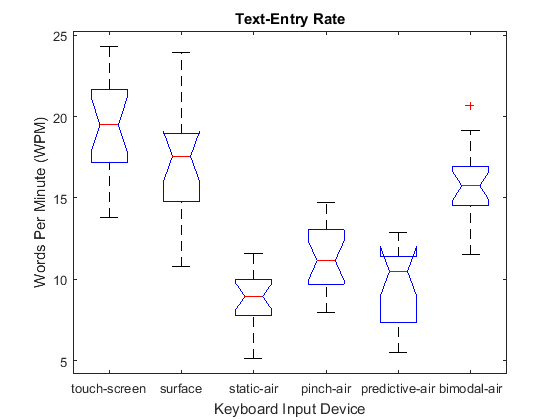
\includegraphics{fig_textentry_boxplot}
	\caption[Text-Entry Rate Boxplot]{Median Text-Entry Rates for each keyboard showing the 25th and 75th percentiles.}
	\label{fig_textentry_boxplot}
\end{figure}

\begin{table}[b]
	\centering
	\caption[Text-Entry Rate Multiple Comparison]{\centering Tukey's Honest Significant Difference with multiple comparison for Text-Entry Rate.}
	\label{textentry_multcompare}
	\resizebox{\textwidth}{!}{\begin{tabular}{ l l r r r r }
		\hline
		\multirow{2}{*}{Group 1} & \multirow{2}{*}{Group 2} & Confidience Interval & Mean Difference & Confidience Interval & \multirow{2}{*}{$p$-value} \\
		{} & {} & Lower End & $\mu_1 - \mu_2$ & Upper End & {} \\
		\hline
		touchscreen & surface & -0.0837 & 2.3522 & 4.7882 & 0.0648 \\
		touchscreen & static-air & 8.4479 & 10.8839 & 13.3198 & 0.0000 \\
		touchscreen & pinch-air & 5.6920 & 8.1280 & 10.5639 & 0.0000 \\
		touchscreen & predictive-air & 7.4227 & 9.8587 & 12.2946 & 0.0000 \\
		touchscreen & bimodal-air & 1.2832 & 3.7192 & 6.1551 & 0.0003 \\
		surface & static-air & 6.0957 & 8.5316 & 10.9676 & 0.0000 \\
		surface & pinch-air & 3.3398 & 5.7757 & 8.2117 & 0.0000 \\
		surface & predictive-air & 5.0705 & 7.5064 & 9.9424 & 0.0000 \\
		surface & bimodal-air & -1.0690 & 1.3669 & 3.8029 & 0.5809 \\
		static-air & pinch-air & -5.1919 & -2.7559 & -0.3199 & 0.0170 \\
		static-air & predictive-air & -3.4612 & -1.0252 & 1.4108 & 0.8249 \\
		static-air & bimodal-air & -9.6007 & -7.1647 & -4.7287 & 0.0000 \\
		pinch-air & predictive-air & -0.7053 & 1.7307 & 4.1667 & 0.3146 \\
		pinch-air & bimodal-air & -6.8448 & -4.4088 & -1.9728 & 0.0000 \\
		predictive-air & bimodal-air & -8.5755 & -6.1395 & -3.7035 & 0.0000 \\
		\hline
	\end{tabular}}
\end{table}

\clearpage
\subsection{Text-Entry Rate Modified-Shortest}
\begin{figure}[h]
	\centering
	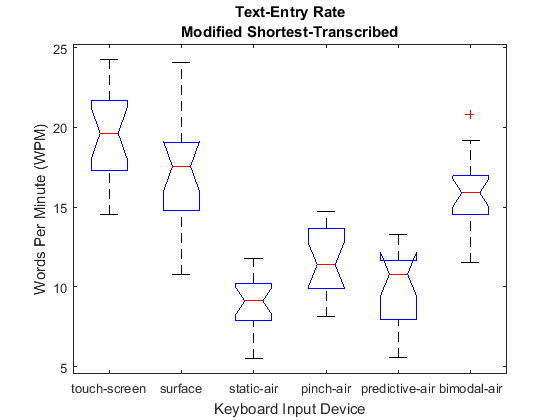
\includegraphics{fig_textentry_short_boxplot}
	\caption[Text-Entry Rates Boxplot for Modified-Shortest]{Median Text-Entry Rates using the shortest-transcribed modification for each keyboard showing the 25th and 75th percentiles.}
	\label{fig_textentry_short_boxplot}
\end{figure}

\begin{table}[h]
\centering
\caption[Text-Entry Rate Multiple Comparison Modified-Shortest]{\centering Tukey's Honest Significant Difference with multiple comparison for Text-Entry Rate modified with shortest-transcribed.}
\label{textentry_short_multcompare}
\resizebox{\textwidth}{!}{\begin{tabular}{ l l r r r r }
\hline
\multirow{2}{*}{Group 1} & \multirow{2}{*}{Group 2} & Confidience Interval & Mean Difference & Confidience Interval & \multirow{2}{*}{$p$-value} \\
{} & {} & Lower End & $\mu_1 - \mu_2$ & Upper End & {} \\
\hline
touchscreen & surface & -0.0162 & 2.4063 & 4.8288 & 0.0526 \\
touchscreen & static-air & 8.4069 & 10.8295 & 13.2520 & 0.0000 \\
touchscreen & pinch-air & 5.6271 & 8.0496 & 10.4722 & 0.0000 \\
touchscreen & predictive-air & 7.3096 & 9.7321 & 12.1546 & 0.0000 \\
touchscreen & bimodal-air & 1.3652 & 3.7877 & 6.2103 & 0.0002 \\
surface & static-air & 6.0006 & 8.4232 & 10.8457 & 0.0000 \\
surface & pinch-air & 3.2208 & 5.6433 & 8.0659 & 0.0000 \\
surface & predictive-air & 4.9033 & 7.3258 & 9.7483 & 0.0000 \\
surface & bimodal-air & -1.0411 & 1.3814 & 3.8040 & 0.5636 \\
static-air & pinch-air & -5.2024 & -2.7798 & -0.3573 & 0.0148 \\
static-air & predictive-air & -3.5199 & -1.0974 & 1.3251 & 0.7757 \\
static-air & bimodal-air & -9.4643 & -7.0417 & -4.6192 & 0.0000 \\
pinch-air & predictive-air & -0.7401 & 1.6825 & 4.1050 & 0.3399 \\
pinch-air & bimodal-air & -6.6844 & -4.2619 & -1.8394 & 0.0000 \\
predictive-air & bimodal-air & -8.3669 & -5.9443 & -3.5218 & 0.0000 \\
\hline
\end{tabular}}
\end{table}

\clearpage
\section{Error Rates}
\subsection{Minimum Word Distance}
\begin{figure}[h]
	\centering
	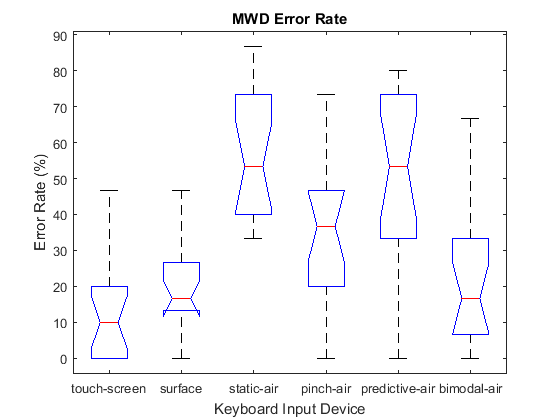
\includegraphics{fig_MWD_boxplot}
	\caption[Minimum Word Distance Boxplot]{Median Minimum Word Distance for each keyboard showing the 25th and 75th percentiles.}
	\label{fig_MWD_boxplot}
\end{figure}

\begin{table}[h]
\centering
\caption[MWD Multiple Comparison]{\centering Tukey's Honest Significant Difference with multiple comparison for Minimum Word Distance.}
\label{MWD_multcompare}
\resizebox{\textwidth}{!}{\begin{tabular}{ l l r r r r }
\hline
\multirow{2}{*}{Group 1} & \multirow{2}{*}{Group 2} & Confidience Interval & Mean Difference & Confidience Interval & \multirow{2}{*}{$p$-value} \\
{} & {} & Lower End & $\mu_1 - \mu_2$ & Upper End & {} \\
\hline
touchscreen & surface & -23.8140 & -5.9259 & 11.9622 & 0.9287 \\
touchscreen & static-air & -61.5918 & -43.7037 & -25.8156 & 0.0000 \\
touchscreen & pinch-air & -39.3696 & -21.4815 & -3.5934 & 0.0091 \\
touchscreen & predictive-air & -53.8140 & -35.9259 & -18.0378 & 0.0000 \\
touchscreen & bimodal-air & -25.2955 & -7.4074 & 10.4807 & 0.8346 \\
surface & static-air & -55.6659 & -37.7778 & -19.8897 & 0.0000 \\
surface & pinch-air & -33.4437 & -15.5556 & 2.3326 & 0.1263 \\
surface & predictive-air & -47.8881 & -30.0000 & -12.1119 & 0.0001 \\
surface & bimodal-air & -19.3696 & -1.4815 & 16.4066 & 0.9999 \\
static-air & pinch-air & 4.3341 & 22.2222 & 40.1103 & 0.0062 \\
static-air & predictive-air & -10.1103 & 7.7778 & 25.6659 & 0.8043 \\
static-air & bimodal-air & 18.4082 & 36.2963 & 54.1844 & 0.0000 \\
pinch-air & predictive-air & -32.3326 & -14.4444 & 3.4437 & 0.1859 \\
pinch-air & bimodal-air & -3.8140 & 14.0741 & 31.9622 & 0.2096 \\
predictive-air & bimodal-air & 10.6304 & 28.5185 & 46.4066 & 0.0002 \\
\hline
\end{tabular}}
\end{table}

\clearpage
\subsubsection{MWD Modified-Shortest}
\begin{figure}[h]
	\centering
	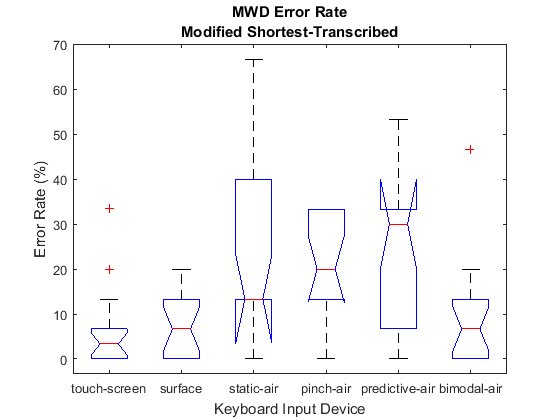
\includegraphics{fig_MWD_short_boxplot}
	\caption[Minimum Word Distance Boxplot for Modified-Shortest]{Median Minimum Word Distance using the shortest-transcribed modification for each keyboard showing the 25th and 75th percentiles.}
	\label{fig_MWD_short_boxplot}
\end{figure}

\begin{table}[h]
\centering
\caption[MWD Multiple Comparison Modified-Shortest]{\centering Tukey's Honest Significant Difference with multiple comparison for Minimum Word Distance using shortest-transcribed modification.}
\label{MWD_short_multcompare}
\resizebox{\textwidth}{!}{\begin{tabular}{ l l r r r r }
\hline
\multirow{2}{*}{Group 1} & \multirow{2}{*}{Group 2} & Confidience Interval & Mean Difference & Confidience Interval & \multirow{2}{*}{$p$-value} \\
{} & {} & Lower End & $\mu_1 - \mu_2$ & Upper End & {} \\
\hline
touchscreen & surface & -13.0458 & 0.0000 & 13.0458 & 1.0000 \\
touchscreen & static-air & -32.3051 & -19.2593 & -6.2135 & 0.0006 \\
touchscreen & pinch-air & -26.7495 & -13.7037 & -0.6579 & 0.0336 \\
touchscreen & predictive-air & -32.6754 & -19.6296 & -6.5838 & 0.0004 \\
touchscreen & bimodal-air & -16.7495 & -3.7037 & 9.3421 & 0.9623 \\
surface & static-air & -32.3051 & -19.2593 & -6.2135 & 0.0006 \\
surface & pinch-air & -26.7495 & -13.7037 & -0.6579 & 0.0336 \\
surface & predictive-air & -32.6754 & -19.6296 & -6.5838 & 0.0004 \\
surface & bimodal-air & -16.7495 & -3.7037 & 9.3421 & 0.9623 \\
static-air & pinch-air & -7.4902 & 5.5556 & 18.6013 & 0.8177 \\
static-air & predictive-air & -13.4162 & -0.3704 & 12.6754 & 1.0000 \\
static-air & bimodal-air & 2.5098 & 15.5556 & 28.6013 & 0.0099 \\
pinch-air & predictive-air & -18.9717 & -5.9259 & 7.1199 & 0.7737 \\
pinch-air & bimodal-air & -3.0458 & 10.0000 & 23.0458 & 0.2349 \\
predictive-air & bimodal-air & 2.8801 & 15.9259 & 28.9717 & 0.0076 \\
\hline
\end{tabular}}
\end{table}

\clearpage
\subsection{Keystrokes Per Character}
\begin{figure}[h]
	\centering
	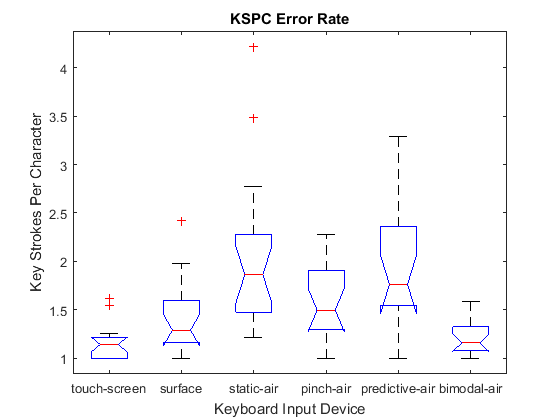
\includegraphics{fig_KSPC_boxplot}
	\caption[Keystrokes Per Character Boxplot]{Median Keystrokes Per Character for each keyboard showing the 25th and 75th percentiles.}
	\label{fig_KSPC_boxplot}
\end{figure}

\begin{table}[h]
\centering
\caption[KSPC Multiple Comparison]{\centering Tukey's Honest Significant Difference with multiple comparison for Keystrokes Per Character.}
\label{KSPC_multcompare}
\resizebox{\textwidth}{!}{\begin{tabular}{ l l r r r r }
\hline
\multirow{2}{*}{Group 1} & \multirow{2}{*}{Group 2} & Confidience Interval & Mean Difference & Confidience Interval & \multirow{2}{*}{$p$-value} \\
{} & {} & Lower End & $\mu_1 - \mu_2$ & Upper End & {} \\
\hline
touchscreen & surface & -0.7298 & -0.2597 & 0.2103 & 0.5972 \\
touchscreen & static-air & -1.3559 & -0.8859 & -0.4158 & 0.0000 \\
touchscreen & pinch-air & -0.8998 & -0.4298 & 0.0403 & 0.0935 \\
touchscreen & predictive-air & -1.2113 & -0.7412 & -0.2712 & 0.0002 \\
touchscreen & bimodal-air & -0.5324 & -0.0623 & 0.4077 & 0.9989 \\
surface & static-air & -1.0962 & -0.6262 & -0.1561 & 0.0026 \\
surface & pinch-air & -0.6401 & -0.1701 & 0.3000 & 0.8993 \\
surface & predictive-air & -0.9515 & -0.4815 & -0.0114 & 0.0414 \\
surface & bimodal-air & -0.2726 & 0.1974 & 0.6675 & 0.8262 \\
static-air & pinch-air & -0.0140 & 0.4561 & 0.9262 & 0.0626 \\
static-air & predictive-air & -0.3254 & 0.1447 & 0.6147 & 0.9471 \\
static-air & bimodal-air & 0.3535 & 0.8236 & 1.2936 & 0.0000 \\
pinch-air & predictive-air & -0.7815 & -0.3114 & 0.1586 & 0.3935 \\
pinch-air & bimodal-air & -0.1026 & 0.3675 & 0.8375 & 0.2157 \\
predictive-air & bimodal-air & 0.2089 & 0.6789 & 1.1490 & 0.0008 \\
\hline
\end{tabular}}
\end{table}

\clearpage
\subsubsection{KSPC Modified-Shortest}
\begin{figure}[h]
	\centering
	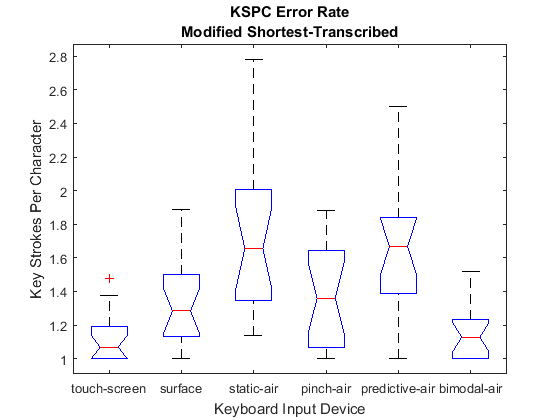
\includegraphics{fig_KSPC_short_boxplot}
	\caption[Keystrokes Per Character Boxplot for Modified-Shortest]{Median Keystrokes Per Character using the shortest-transcribed modification for each keyboard showing the 25th and 75th percentiles.}
	\label{fig_KSPC_short_boxplot}
\end{figure}

\begin{table}[h]
\centering
\caption[KSPC Multiple Comparison Modified-Shortest]{\centering Tukey's Honest Significant Difference with multiple comparison for Keystrokes Per Character using shortest-transcribed modification.}
\label{KSPC_short_multcompare}
\resizebox{\textwidth}{!}{\begin{tabular}{ l l r r r r }
\hline
\multirow{2}{*}{Group 1} & \multirow{2}{*}{Group 2} & Confidience Interval & Mean Difference & Confidience Interval & \multirow{2}{*}{$p$-value} \\
{} & {} & Lower End & $\mu_1 - \mu_2$ & Upper End & {} \\
\hline
touchscreen & surface & -0.5181 & -0.2055 & 0.1070 & 0.4020 \\
touchscreen & static-air & -0.9366 & -0.6240 & -0.3115 & 0.0000 \\
touchscreen & pinch-air & -0.5532 & -0.2407 & 0.0719 & 0.2304 \\
touchscreen & predictive-air & -0.8488 & -0.5363 & -0.2237 & 0.0000 \\
touchscreen & bimodal-air & -0.3346 & -0.0220 & 0.2906 & 0.9999 \\
surface & static-air & -0.7310 & -0.4185 & -0.1059 & 0.0024 \\
surface & pinch-air & -0.3477 & -0.0351 & 0.2774 & 0.9995 \\
surface & predictive-air & -0.6433 & -0.3307 & -0.0182 & 0.0316 \\
surface & bimodal-air & -0.1290 & 0.1835 & 0.4961 & 0.5313 \\
static-air & pinch-air & 0.0708 & 0.3833 & 0.6959 & 0.0072 \\
static-air & predictive-air & -0.2248 & 0.0877 & 0.4003 & 0.9641 \\
static-air & bimodal-air & 0.2895 & 0.6020 & 0.9146 & 0.0000 \\
pinch-air & predictive-air & -0.6082 & -0.2956 & 0.0169 & 0.0748 \\
pinch-air & bimodal-air & -0.0939 & 0.2187 & 0.5312 & 0.3316 \\
predictive-air & bimodal-air & 0.2017 & 0.5143 & 0.8269 & 0.0001 \\
\hline
\end{tabular}}
\end{table}

\clearpage
\subsection{Minimum String Distance}
\subsubsection{MSD Modified-Shortest}
\begin{figure}[h]
	\centering
	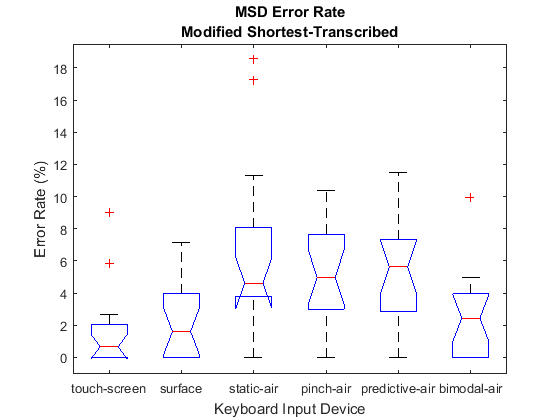
\includegraphics{fig_MSD_short_boxplot}
	\caption[Minimum String Distance Boxplot for Modified-Shortest]{Median Minimum String Distance using the shortest-transcribed modification for each keyboard showing the 25th and 75th percentiles.}
	\label{fig_MSD_short_boxplot}
\end{figure}

\begin{table}[h]
\centering
\caption[MSD Multiple Comparison Modified-Shortest]{\centering Tukey's Honest Significant Difference with multiple comparison for Minimum String Distance using shortest-transcribed modification.}
\label{MSD_short_multcompare}
\resizebox{\textwidth}{!}{\begin{tabular}{ l l r r r r }
\hline
\multirow{2}{*}{Group 1} & \multirow{2}{*}{Group 2} & Confidience Interval & Mean Difference & Confidience Interval & \multirow{2}{*}{$p$-value} \\
{} & {} & Lower End & $\mu_1 - \mu_2$ & Upper End & {} \\
\hline
touchscreen & surface & -3.7747 & -0.6145 & 2.5457 & 0.9931 \\
touchscreen & static-air & -7.9973 & -4.8372 & -1.6770 & 0.0003 \\
touchscreen & pinch-air & -6.7038 & -3.5437 & -0.3835 & 0.0186 \\
touchscreen & predictive-air & -6.9953 & -3.8351 & -0.6749 & 0.0081 \\
touchscreen & bimodal-air & -4.0980 & -0.9378 & 2.2223 & 0.9546 \\
surface & static-air & -7.3828 & -4.2227 & -1.0625 & 0.0025 \\
surface & pinch-air & -6.0893 & -2.9292 & 0.2310 & 0.0856 \\
surface & predictive-air & -6.3808 & -3.2206 & -0.0604 & 0.0431 \\
surface & bimodal-air & -3.4835 & -0.3233 & 2.8368 & 0.9997 \\
static-air & pinch-air & -1.8667 & 1.2935 & 4.4537 & 0.8412 \\
static-air & predictive-air & -2.1581 & 1.0021 & 4.1622 & 0.9403 \\
static-air & bimodal-air & 0.7392 & 3.8993 & 7.0595 & 0.0067 \\
pinch-air & predictive-air & -3.4516 & -0.2914 & 2.8687 & 0.9998 \\
pinch-air & bimodal-air & -0.5543 & 2.6058 & 5.7660 & 0.1677 \\
predictive-air & bimodal-air & -0.2629 & 2.8973 & 6.0574 & 0.0919 \\
\hline
\end{tabular}}
\end{table}

\clearpage
\subsection{Total Error Rate}
\begin{figure}[h]
	\centering
	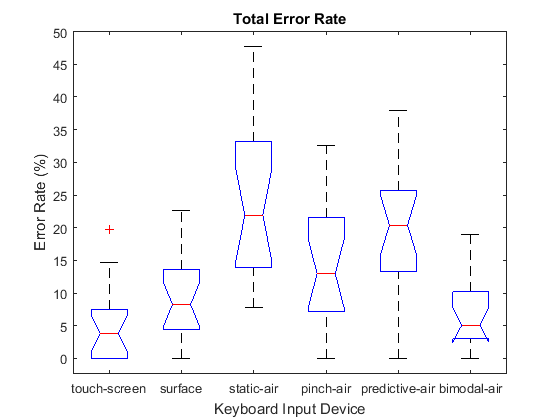
\includegraphics{fig_totER_boxplot}
	\caption[Total Error Rate Boxplot]{Median Total Error Rate for each keyboard showing the 25th and 75th percentiles.}
	\label{fig_totER_boxplot}
\end{figure}

\begin{table}[h]
\centering
\caption[Total Error Rate Multiple Comparison]{\centering Tukey's Honest Significant Difference with multiple comparison for Total Error Rate.}
\label{totER_multcompare}
\resizebox{\textwidth}{!}{\begin{tabular}{ l l r r r r }
\hline
\multirow{2}{*}{Group 1} & \multirow{2}{*}{Group 2} & Confidience Interval & Mean Difference & Confidience Interval & \multirow{2}{*}{$p$-value} \\
{} & {} & Lower End & $\mu_1 - \mu_2$ & Upper End & {} \\
\hline
touchscreen & surface & -12.9197 & -4.3716 & 4.1766 & 0.6743 \\
touchscreen & static-air & -27.2196 & -18.6714 & -10.1233 & 0.0000 \\
touchscreen & pinch-air & -17.6640 & -9.1158 & -0.5677 & 0.0295 \\
touchscreen & predictive-air & -23.6696 & -15.1214 & -6.5733 & 0.0000 \\
touchscreen & bimodal-air & -10.4357 & -1.8875 & 6.6606 & 0.9875 \\
surface & static-air & -22.8480 & -14.2999 & -5.7517 & 0.0001 \\
surface & pinch-air & -13.2924 & -4.7443 & 3.8039 & 0.5926 \\
surface & predictive-air & -19.2980 & -10.7498 & -2.2017 & 0.0054 \\
surface & bimodal-air & -6.0641 & 2.4840 & 11.0322 & 0.9584 \\
static-air & pinch-air & 1.0075 & 9.5556 & 18.1038 & 0.0191 \\
static-air & predictive-air & -4.9981 & 3.5500 & 12.0982 & 0.8329 \\
static-air & bimodal-air & 8.2358 & 16.7839 & 25.3321 & 0.0000 \\
pinch-air & predictive-air & -14.5537 & -6.0056 & 2.5425 & 0.3270 \\
pinch-air & bimodal-air & -1.3198 & 7.2283 & 15.7764 & 0.1473 \\
predictive-air & bimodal-air & 4.6858 & 13.2339 & 21.7820 & 0.0003 \\
\hline
\end{tabular}}
\end{table}

\clearpage
\subsubsection{Total Error Rate Modified-Shortest}
\begin{figure}[h]
	\centering
	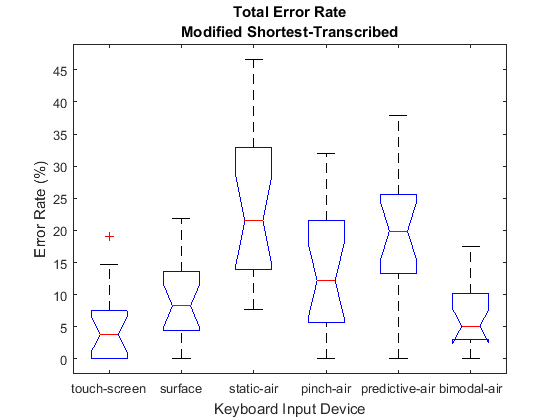
\includegraphics{fig_totER_short_boxplot}
	\caption[Total Error Rate Boxplot for Modified-Shortest]{Median Total Error Rate using the shortest-transcribed modification for each keyboard showing the 25th and 75th percentiles.}
	\label{fig_totER_short_boxplot}
\end{figure}

\begin{table}[h]
\centering
\caption[Total Error Rate Multiple Comparison Modified-Shortest]{\centering Tukey's Honest Significant Difference with multiple comparison for Total Error Rate using shortest-transcribed modification.}
\label{totER_short_multcompare}
\resizebox{\textwidth}{!}{\begin{tabular}{ l l r r r r }
\hline
\multirow{2}{*}{Group 1} & \multirow{2}{*}{Group 2} & Confidience Interval & Mean Difference & Confidience Interval & \multirow{2}{*}{$p$-value} \\
{} & {} & Lower End & $\mu_1 - \mu_2$ & Upper End & {} \\
\hline
touchscreen & surface & -12.6316 & -4.3367 & 3.9581 & 0.6532 \\
touchscreen & static-air & -26.7322 & -18.4374 & -10.1426 & 0.0000 \\
touchscreen & pinch-air & -16.8635 & -8.5686 & -0.2738 & 0.0386 \\
touchscreen & predictive-air & -22.7732 & -14.4783 & -6.1835 & 0.0000 \\
touchscreen & bimodal-air & -10.1405 & -1.8456 & 6.4492 & 0.9871 \\
surface & static-air & -22.3955 & -14.1007 & -5.8058 & 0.0000 \\
surface & pinch-air & -12.5268 & -4.2319 & 4.0629 & 0.6765 \\
surface & predictive-air & -18.4364 & -10.1416 & -1.8468 & 0.0075 \\
surface & bimodal-air & -5.8037 & 2.4911 & 10.7859 & 0.9523 \\
static-air & pinch-air & 1.5739 & 9.8688 & 18.1636 & 0.0101 \\
static-air & predictive-air & -4.3358 & 3.9591 & 12.2539 & 0.7351 \\
static-air & bimodal-air & 8.2969 & 16.5918 & 24.8866 & 0.0000 \\
pinch-air & predictive-air & -14.2045 & -5.9097 & 2.3851 & 0.3116 \\
pinch-air & bimodal-air & -1.5718 & 6.7230 & 15.0178 & 0.1826 \\
predictive-air & bimodal-air & 4.3379 & 12.6327 & 20.9275 & 0.0003 \\
\hline
\end{tabular}}
\end{table}

\clearpage
\section{Correctness}
\subsection{Fr\'echet Distance}
\begin{figure}[h]
	\centering
	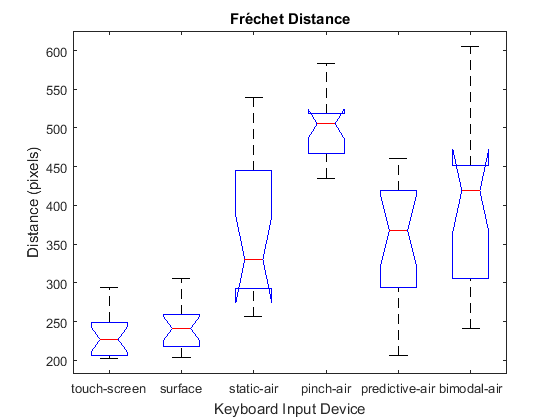
\includegraphics{fig_frechet_boxplot}
	\caption[Fr\'echet Distance Boxplot]{Median Fr\'echet Distance for each keyboard showing the 25th and 75th percentiles.}
	\label{fig_frechet_boxplot}
\end{figure}

\begin{table}[h]
\centering
\caption[Fr\'echet Distance Multiple Comparison]{\centering Tukey's Honest Significant Difference with multiple comparison for Fr\'echet Distance.}
\label{frechet_multcompare}
\resizebox{\textwidth}{!}{\begin{tabular}{ l l r r r r }
\hline
\multirow{2}{*}{Group 1} & \multirow{2}{*}{Group 2} & Confidience Interval & Mean Difference & Confidience Interval & \multirow{2}{*}{$p$-value} \\
{} & {} & Lower End & $\mu_1 - \mu_2$ & Upper End & {} \\
\hline
touchscreen & surface & -78.8540 & -11.6328 & 55.5884 & 0.9960 \\
touchscreen & static-air & -200.3012 & -133.0800 & -65.8588 & 0.0000 \\
touchscreen & pinch-air & -337.2356 & -270.0144 & -202.7931 & 0.0000 \\
touchscreen & predictive-air & -186.6273 & -119.4061 & -52.1849 & 0.0000 \\
touchscreen & bimodal-air & -232.5464 & -165.3252 & -98.1040 & 0.0000 \\
surface & static-air & -188.6684 & -121.4472 & -54.2260 & 0.0000 \\
surface & pinch-air & -325.6027 & -258.3815 & -191.1603 & 0.0000 \\
surface & predictive-air & -174.9945 & -107.7733 & -40.5521 & 0.0001 \\
surface & bimodal-air & -220.9136 & -153.6924 & -86.4712 & 0.0000 \\
static-air & pinch-air & -204.1555 & -136.9343 & -69.7131 & 0.0000 \\
static-air & predictive-air & -53.5473 & 13.6739 & 80.8951 & 0.9914 \\
static-air & bimodal-air & -99.4664 & -32.2452 & 34.9760 & 0.7309 \\
pinch-air & predictive-air & 83.3870 & 150.6083 & 217.8295 & 0.0000 \\
pinch-air & bimodal-air & 37.4679 & 104.6891 & 171.9103 & 0.0002 \\
predictive-air & bimodal-air & -113.1403 & -45.9191 & 21.3021 & 0.3586 \\
\hline
\end{tabular}}
\end{table}

\clearpage
\subsubsection{Fr\'echet Distance Modified-Shortest}
\begin{figure}[h]
	\centering
	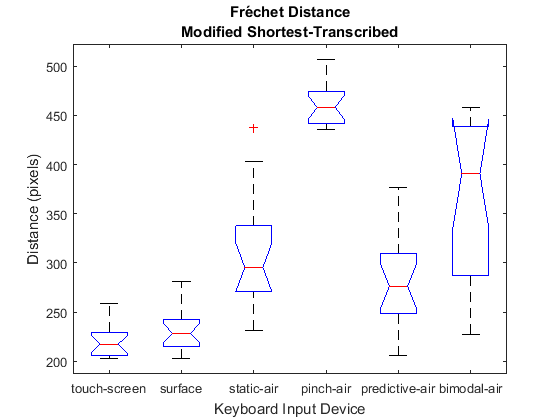
\includegraphics{fig_frechet_short_boxplot}
	\caption[Fr\'echet Distance Boxplot for Modified-Shortest]{Median Fr\'echet Distance using the shortest-transcribed modification for each keyboard showing the 25th and 75th percentiles.}
	\label{fig_frechet_short_boxplot}
\end{figure}

\begin{table}[h]
\centering
\caption[Fr\'echet Distance Multiple Comparison Modified-Shortest]{\centering Tukey's Honest Significant Difference with multiple comparison for Fr\'echet Distance using shortest-transcribed modification.}
\label{frechet_short_multcompare}
\resizebox{\textwidth}{!}{\begin{tabular}{ l l r r r r }
\hline
\multirow{2}{*}{Group 1} & \multirow{2}{*}{Group 2} & Confidience Interval & Mean Difference & Confidience Interval & \multirow{2}{*}{$p$-value} \\
{} & {} & Lower End & $\mu_1 - \mu_2$ & Upper End & {} \\
\hline
touchscreen & surface & -55.6656 & -9.9934 & 35.6788 & 0.9881 \\
touchscreen & static-air & -131.1279 & -85.4556 & -39.7834 & 0.0000 \\
touchscreen & pinch-air & -283.8592 & -238.1870 & -192.5147 & 0.0000 \\
touchscreen & predictive-air & -106.2951 & -60.6229 & -14.9506 & 0.0027 \\
touchscreen & bimodal-air & -193.0612 & -147.3890 & -101.7167 & 0.0000 \\
surface & static-air & -121.1345 & -75.4622 & -29.7900 & 0.0001 \\
surface & pinch-air & -273.8658 & -228.1936 & -182.5213 & 0.0000 \\
surface & predictive-air & -96.3017 & -50.6295 & -4.9572 & 0.0207 \\
surface & bimodal-air & -183.0678 & -137.3956 & -91.7233 & 0.0000 \\
static-air & pinch-air & -198.4036 & -152.7313 & -107.0591 & 0.0000 \\
static-air & predictive-air & -20.8395 & 24.8328 & 70.5050 & 0.6140 \\
static-air & bimodal-air & -107.6056 & -61.9333 & -16.2611 & 0.0020 \\
pinch-air & predictive-air & 131.8919 & 177.5641 & 223.2363 & 0.0000 \\
pinch-air & bimodal-air & 45.1258 & 90.7980 & 136.4702 & 0.0000 \\
predictive-air & bimodal-air & -132.4383 & -86.7661 & -41.0939 & 0.0000 \\
\hline
\end{tabular}}
\end{table}

\clearpage
\subsubsection{Fr\'echet Distance Modified-Backspace}
\begin{figure}[h]
	\centering
	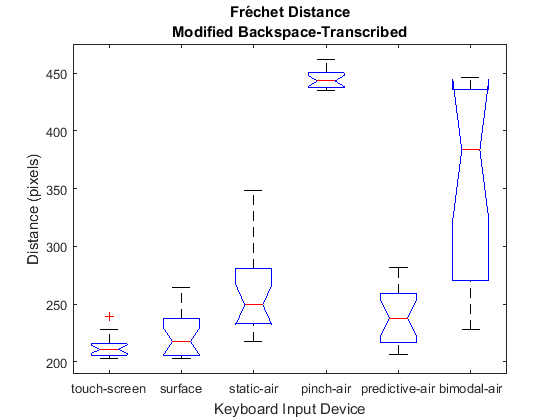
\includegraphics{fig_frechet_back_boxplot}
	\caption[Fr\'echet Distance Boxplot for Modified-Backspace]{Median Fr\'echet Distance using the backspace-transcribed modification for each keyboard showing the 25th and 75th percentiles.}
	\label{fig_frechet_back_boxplot}
\end{figure}

\begin{table}[h]
\centering
\caption[Fr\'echet Distance Multiple Comparison Modified-Backspace]{\centering Tukey's Honest Significant Difference with multiple comparison for Fr\'echet Distance using backspace-transcribed modification.}
\label{frechet_back_multcompare}
\resizebox{\textwidth}{!}{\begin{tabular}{ l l r r r r }
\hline
\multirow{2}{*}{Group 1} & \multirow{2}{*}{Group 2} & Confidience Interval & Mean Difference & Confidience Interval & \multirow{2}{*}{$p$-value} \\
{} & {} & Lower End & $\mu_1 - \mu_2$ & Upper End & {} \\
\hline
touchscreen & surface & -49.6728 & -11.2179 & 27.2370 & 0.9577 \\
touchscreen & static-air & -85.0013 & -46.5465 & -8.0916 & 0.0084 \\
touchscreen & pinch-air & -270.8703 & -232.4155 & -193.9606 & 0.0000 \\
touchscreen & predictive-air & -63.8306 & -25.3757 & 13.0791 & 0.3981 \\
touchscreen & bimodal-air & -182.9460 & -144.4911 & -106.0363 & 0.0000 \\
surface & static-air & -73.7834 & -35.3285 & 3.1263 & 0.0907 \\
surface & pinch-air & -259.6524 & -221.1975 & -182.7427 & 0.0000 \\
surface & predictive-air & -52.6127 & -14.1578 & 24.2970 & 0.8924 \\
surface & bimodal-air & -171.7281 & -133.2732 & -94.8183 & 0.0000 \\
static-air & pinch-air & -224.3239 & -185.8690 & -147.4141 & 0.0000 \\
static-air & predictive-air & -17.2842 & 21.1707 & 59.6256 & 0.6011 \\
static-air & bimodal-air & -136.3995 & -97.9447 & -59.4898 & 0.0000 \\
pinch-air & predictive-air & 168.5848 & 207.0397 & 245.4946 & 0.0000 \\
pinch-air & bimodal-air & 49.4694 & 87.9243 & 126.3792 & 0.0000 \\
predictive-air & bimodal-air & -157.5703 & -119.1154 & -80.6605 & 0.0000 \\
\hline
\end{tabular}}
\end{table}

\clearpage
\section{Distance Measures}
\subsection{Word-Gesture Distance}
\begin{figure}[h]
	\centering
	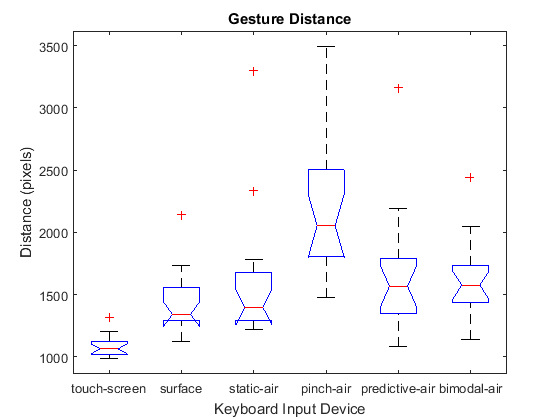
\includegraphics{fig_distance_boxplot}
	\caption[Word-Gesture Distance Boxplot]{Median Word-Gesture Distance for each keyboard showing the 25th and 75th percentiles.}
	\label{fig_distance_boxplot}
\end{figure}

\begin{table}[h]
\centering
\caption[Word-Gesture Distance Multiple Comparison]{\centering Tukey's Honest Significant Difference with multiple comparison for Word-Gesture Distance.}
\label{distance_multcompare}
\resizebox{\textwidth}{!}{\begin{tabular}{ l l r r r r }
\hline
\multirow{2}{*}{Group 1} & \multirow{2}{*}{Group 2} & Confidience Interval & Mean Difference & Confidience Interval & \multirow{2}{*}{$p$-value} \\
{} & {} & Lower End & $\mu_1 - \mu_2$ & Upper End & {} \\
\hline
touchscreen & surface & -722.3100 & -336.4100 & 49.4910 & 0.1245 \\
touchscreen & static-air & -889.2300 & -503.3300 & -117.4300 & 0.0034 \\
touchscreen & pinch-air & -1463.6000 & -1077.7000 & -691.8200 & 0.0000 \\
touchscreen & predictive-air & -933.1100 & -547.2100 & -161.3100 & 0.0011 \\
touchscreen & bimodal-air & -926.0700 & -540.1700 & -154.2700 & 0.0013 \\
surface & static-air & -552.8200 & -166.9200 & 218.9800 & 0.8077 \\
surface & pinch-air & -1127.2000 & -741.3100 & -355.4100 & 0.0000 \\
surface & predictive-air & -596.7000 & -210.8000 & 175.1000 & 0.6092 \\
surface & bimodal-air & -589.6600 & -203.7600 & 182.1500 & 0.6435 \\
static-air & pinch-air & -960.3000 & -574.3900 & -188.4900 & 0.0005 \\
static-air & predictive-air & -429.7800 & -43.8820 & 342.0200 & 0.9995 \\
static-air & bimodal-air & -422.7400 & -36.8390 & 349.0600 & 0.9998 \\
pinch-air & predictive-air & 144.6100 & 530.5100 & 916.4100 & 0.0017 \\
pinch-air & bimodal-air & 151.6500 & 537.5500 & 923.4600 & 0.0014 \\
predictive-air & bimodal-air & -378.8600 & 7.0433 & 392.9400 & 1.0000 \\
\hline
\end{tabular}}
\end{table}

\clearpage
\subsubsection{Word-Gesture Distance Modified-Shortest}
\begin{figure}[h]
	\centering
	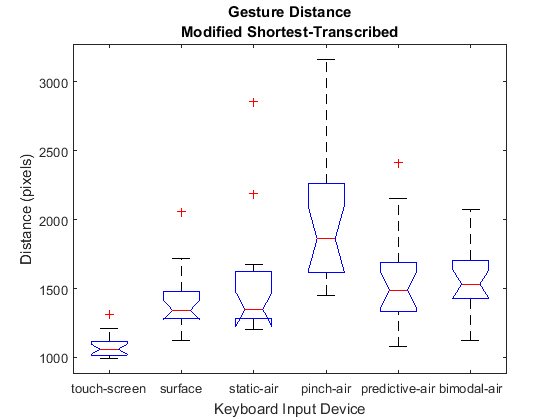
\includegraphics{fig_distance_short_boxplot}
	\caption[Word-Gesture Distance Boxplot for Modified-Shortest]{Median Word-Gesture Distance using the shortest-transcribed modification for each keyboard showing the 25th and 75th percentiles.}
	\label{fig_distance_short_boxplot}
\end{figure}

\begin{table}[h]
\centering
\caption[Word-Gesture Distance Multiple Comparison Modified-Shortest]{\centering Tukey's Honest Significant Difference with multiple comparison for Word-Gesture Distance using shortest-transcribed modification.}
\label{distance_short_multcompare}
\resizebox{\textwidth}{!}{\begin{tabular}{ l l r r r r }
\hline
\multirow{2}{*}{Group 1} & \multirow{2}{*}{Group 2} & Confidience Interval & Mean Difference & Confidience Interval & \multirow{2}{*}{$p$-value} \\
{} & {} & Lower End & $\mu_1 - \mu_2$ & Upper End & {} \\
\hline
touchscreen & surface & -630.0100 & -315.2300 & -0.4611 & 0.0494 \\
touchscreen & static-air & -758.2800 & -443.5100 & -128.7300 & 0.0012 \\
touchscreen & pinch-air & -1214.9000 & -900.1000 & -585.3300 & 0.0000 \\
touchscreen & predictive-air & -770.2100 & -455.4400 & -140.6600 & 0.0008 \\
touchscreen & bimodal-air & -799.9600 & -485.1900 & -170.4200 & 0.0003 \\
surface & static-air & -443.0400 & -128.2700 & 186.5000 & 0.8437 \\
surface & pinch-air & -899.6400 & -584.8700 & -270.0900 & 0.0000 \\
surface & predictive-air & -454.9800 & -140.2000 & 174.5700 & 0.7878 \\
surface & bimodal-air & -484.7300 & -169.9600 & 144.8200 & 0.6211 \\
static-air & pinch-air & -771.3700 & -456.6000 & -141.8200 & 0.0008 \\
static-air & predictive-air & -326.7100 & -11.9330 & 302.8400 & 1.0000 \\
static-air & bimodal-air & -356.4600 & -41.6840 & 273.0900 & 0.9989 \\
pinch-air & predictive-air & 129.8900 & 444.6600 & 759.4400 & 0.0011 \\
pinch-air & bimodal-air & 100.1400 & 414.9100 & 729.6900 & 0.0030 \\
predictive-air & bimodal-air & -344.5200 & -29.7520 & 285.0200 & 0.9998 \\
\hline
\end{tabular}}
\end{table}

\clearpage
\subsection{Word-Gesture Velocity}
\begin{figure}[h]
	\centering
	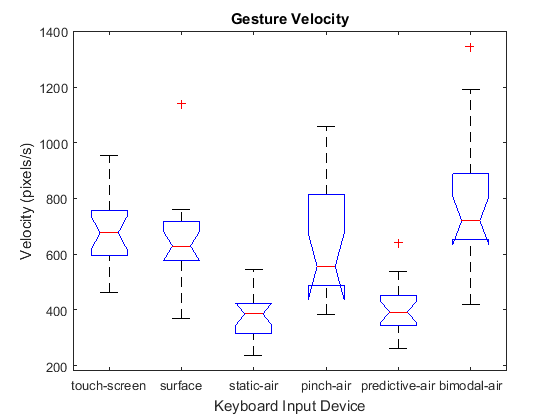
\includegraphics{fig_velocity_gesture_boxplot}
	\caption[Word-Gesture Velocity Boxplot]{Median Word-Gesture Velocity for each keyboard showing the 25th and 75th percentiles.}
	\label{fig_velocity_gesture_boxplot}
\end{figure}

\begin{table}[h]
\centering
\caption[Word-Gesture Velocity Multiple Comparison]{\centering Tukey's Honest Significant Difference with multiple comparison for Word-Gesture Velocity.}
\label{velocity_gesture_multcompare}
\resizebox{\textwidth}{!}{\begin{tabular}{ l l r r r r }
\hline
\multirow{2}{*}{Group 1} & \multirow{2}{*}{Group 2} & Confidience Interval & Mean Difference & Confidience Interval & \multirow{2}{*}{$p$-value} \\
{} & {} & Lower End & $\mu_1 - \mu_2$ & Upper End & {} \\
\hline
touchscreen & surface & -124.4400 & 32.2030 & 188.8500 & 0.9910 \\
touchscreen & static-air & 135.7300 & 292.3800 & 449.0200 & 0.0000 \\
touchscreen & pinch-air & -127.1800 & 29.4680 & 186.1200 & 0.9940 \\
touchscreen & predictive-air & 111.0400 & 267.6900 & 424.3400 & 0.0000 \\
touchscreen & bimodal-air & -260.9500 & -104.3100 & 52.3400 & 0.3877 \\
surface & static-air & 103.5300 & 260.1700 & 416.8200 & 0.0001 \\
surface & pinch-air & -159.3800 & -2.7346 & 153.9100 & 1.0000 \\
surface & predictive-air & 78.8390 & 235.4900 & 392.1300 & 0.0004 \\
surface & bimodal-air & -293.1600 & -136.5100 & 20.1370 & 0.1248 \\
static-air & pinch-air & -419.5500 & -262.9100 & -106.2600 & 0.0001 \\
static-air & predictive-air & -181.3300 & -24.6870 & 131.9600 & 0.9974 \\
static-air & bimodal-air & -553.3300 & -396.6800 & -240.0400 & 0.0000 \\
pinch-air & predictive-air & 81.5740 & 238.2200 & 394.8700 & 0.0004 \\
pinch-air & bimodal-air & -290.4200 & -133.7800 & 22.8720 & 0.1397 \\
predictive-air & bimodal-air & -528.6400 & -372.0000 & -215.3500 & 0.0000 \\
\hline
\end{tabular}}
\end{table}

\clearpage
\subsection{Hand Velocity}
\begin{figure}[h]
	\centering
	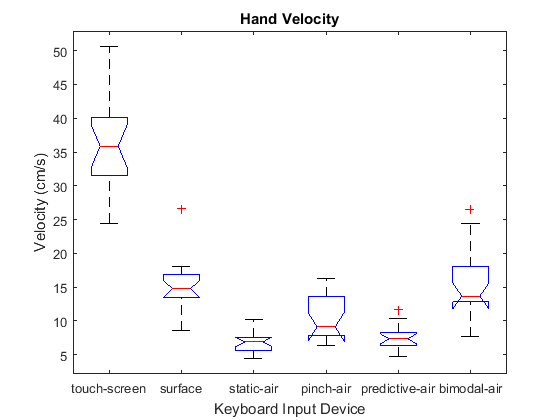
\includegraphics{fig_velocity_hand_boxplot}
	\caption[Hand Velocity Boxplot]{Median Hand Velocity for each keyboard showing the 25th and 75th percentiles.}
	\label{fig_velocity_hand_boxplot}
\end{figure}

\begin{table}[h]
\centering
\caption[Hand Velocity Multiple Comparison]{\centering Tukey's Honest Significant Difference with multiple comparison for Hand Velocity.}
\label{velocity_hand_multcompare}
\resizebox{\textwidth}{!}{\begin{tabular}{ l l r r r r }
\hline
\multirow{2}{*}{Group 1} & \multirow{2}{*}{Group 2} & Confidience Interval & Mean Difference & Confidience Interval & \multirow{2}{*}{$p$-value} \\
{} & {} & Lower End & $\mu_1 - \mu_2$ & Upper End & {} \\
\hline
touchscreen & surface & 16.7046 & 20.6775 & 24.6504 & 0.0000 \\
touchscreen & static-air & 24.8793 & 28.8522 & 32.8251 & 0.0000 \\
touchscreen & pinch-air & 21.2448 & 25.2177 & 29.1906 & 0.0000 \\
touchscreen & predictive-air & 24.1600 & 28.1329 & 32.1058 & 0.0000 \\
touchscreen & bimodal-air & 16.5779 & 20.5508 & 24.5237 & 0.0000 \\
surface & static-air & 4.2018 & 8.1747 & 12.1476 & 0.0000 \\
surface & pinch-air & 0.5673 & 4.5403 & 8.5132 & 0.0154 \\
surface & predictive-air & 3.4825 & 7.4554 & 11.4284 & 0.0000 \\
surface & bimodal-air & -4.0996 & -0.1267 & 3.8462 & 1.0000 \\
static-air & pinch-air & -7.6074 & -3.6345 & 0.3385 & 0.0932 \\
static-air & predictive-air & -4.6922 & -0.7193 & 3.2536 & 0.9950 \\
static-air & bimodal-air & -12.2743 & -8.3014 & -4.3285 & 0.0000 \\
pinch-air & predictive-air & -1.0577 & 2.9152 & 6.8881 & 0.2798 \\
pinch-air & bimodal-air & -8.6399 & -4.6670 & -0.6940 & 0.0116 \\
predictive-air & bimodal-air & -11.5551 & -7.5821 & -3.6092 & 0.0000 \\
\hline
\end{tabular}}
\end{table}

\clearpage
\section{Timing Measures}
\subsection{Word-Gesture Duration}
\begin{figure}[h]
	\centering
	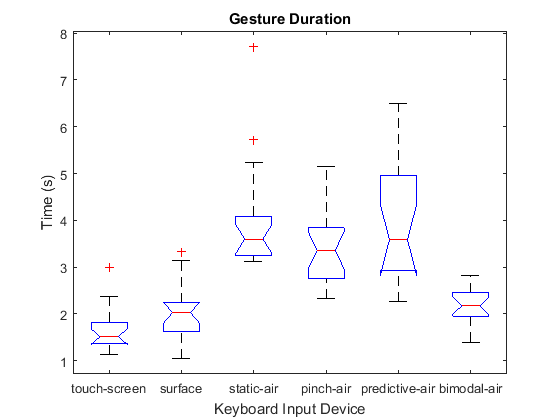
\includegraphics{fig_time_boxplot}
	\caption[Word-Gesture Duration Boxplot]{Median Word-Gesture Duration for each keyboard showing the 25th and 75th percentiles.}
	\label{fig_time_boxplot}
\end{figure}

\begin{table}[h]
\centering
\caption[Word-Gesture Duration Multiple Comparison]{\centering Tukey's Honest Significant Difference with multiple comparison for Word-Gesture Duration.}
\label{time_multcompare}
\resizebox{\textwidth}{!}{\begin{tabular}{ l l r r r r }
\hline
\multirow{2}{*}{Group 1} & \multirow{2}{*}{Group 2} & Confidience Interval & Mean Difference & Confidience Interval & \multirow{2}{*}{$p$-value} \\
{} & {} & Lower End & $\mu_1 - \mu_2$ & Upper End & {} \\
\hline
touchscreen & surface & -1.1732 & -0.3842 & 0.4047 & 0.7181 \\
touchscreen & static-air & -3.1457 & -2.3568 & -1.5679 & 0.0000 \\
touchscreen & pinch-air & -2.5019 & -1.7130 & -0.9241 & 0.0000 \\
touchscreen & predictive-air & -3.0051 & -2.2162 & -1.4272 & 0.0000 \\
touchscreen & bimodal-air & -1.3204 & -0.5315 & 0.2574 & 0.3743 \\
surface & static-air & -2.7615 & -1.9726 & -1.1836 & 0.0000 \\
surface & pinch-air & -2.1177 & -1.3288 & -0.5398 & 0.0001 \\
surface & predictive-air & -2.6208 & -1.8319 & -1.0430 & 0.0000 \\
surface & bimodal-air & -0.9362 & -0.1473 & 0.6417 & 0.9943 \\
static-air & pinch-air & -0.1451 & 0.6438 & 1.4327 & 0.1766 \\
static-air & predictive-air & -0.6483 & 0.1406 & 0.9296 & 0.9954 \\
static-air & bimodal-air & 1.0364 & 1.8253 & 2.6142 & 0.0000 \\
pinch-air & predictive-air & -1.2921 & -0.5031 & 0.2858 & 0.4373 \\
pinch-air & bimodal-air & 0.3926 & 1.1815 & 1.9704 & 0.0005 \\
predictive-air & bimodal-air & 0.8957 & 1.6847 & 2.4736 & 0.0000 \\
\hline
\end{tabular}}
\end{table}

\clearpage
\subsubsection{Word-Gesture Duration Modified-Shortest}
\begin{figure}[h]
	\centering
	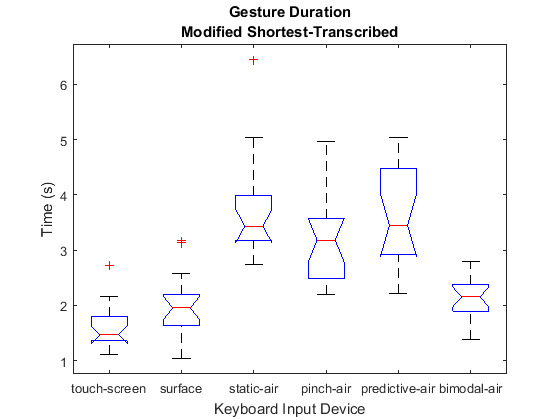
\includegraphics{fig_time_short_boxplot}
	\caption[Word-Gesture Duration Boxplot for Modified-Shortest]{Median Word-Gesture Duration using the shortest-transcribed modification for each keyboard showing the 25th and 75th percentiles.}
	\label{fig_time_short_boxplot}
\end{figure}

\begin{table}[h]
\centering
\caption[Word-Gesture Duration Multiple Comparison Modified-Shortest]{\centering Tukey's Honest Significant Difference with multiple comparison for Word-Gesture Duration using shortest-transcribed modification.}
\label{time_short_multcompare}
\resizebox{\textwidth}{!}{\begin{tabular}{ l l r r r r }
\hline
\multirow{2}{*}{Group 1} & \multirow{2}{*}{Group 2} & Confidience Interval & Mean Difference & Confidience Interval & \multirow{2}{*}{$p$-value} \\
{} & {} & Lower End & $\mu_1 - \mu_2$ & Upper End & {} \\
\hline
touchscreen & surface & -1.0464 & -0.3939 & 0.2587 & 0.5004 \\
touchscreen & static-air & -2.7937 & -2.1411 & -1.4885 & 0.0000 \\
touchscreen & pinch-air & -2.2167 & -1.5641 & -0.9115 & 0.0000 \\
touchscreen & predictive-air & -2.6087 & -1.9561 & -1.3036 & 0.0000 \\
touchscreen & bimodal-air & -1.2034 & -0.5508 & 0.1018 & 0.1488 \\
surface & static-air & -2.3998 & -1.7472 & -1.0947 & 0.0000 \\
surface & pinch-air & -1.8228 & -1.1702 & -0.5177 & 0.0000 \\
surface & predictive-air & -2.2148 & -1.5623 & -0.9097 & 0.0000 \\
surface & bimodal-air & -0.8095 & -0.1569 & 0.4957 & 0.9817 \\
static-air & pinch-air & -0.0756 & 0.5770 & 1.2296 & 0.1147 \\
static-air & predictive-air & -0.4676 & 0.1850 & 0.8375 & 0.9626 \\
static-air & bimodal-air & 0.9378 & 1.5903 & 2.2429 & 0.0000 \\
pinch-air & predictive-air & -1.0446 & -0.3920 & 0.2605 & 0.5058 \\
pinch-air & bimodal-air & 0.3608 & 1.0133 & 1.6659 & 0.0002 \\
predictive-air & bimodal-air & 0.7528 & 1.4054 & 2.0579 & 0.0000 \\
\hline
\end{tabular}}
\end{table}

\clearpage
\subsection{Reaction Time to Errors}
\begin{figure}[h]
	\centering
	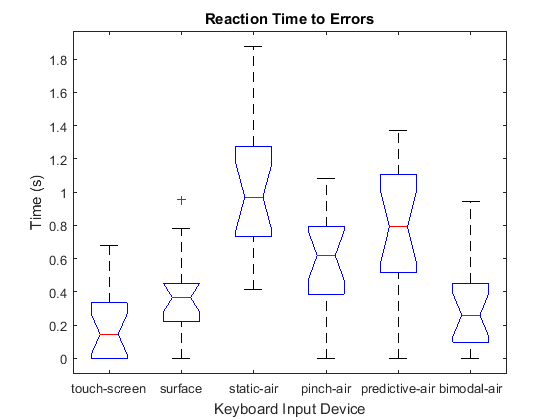
\includegraphics{fig_reaction_errors_boxplot}
	\caption[Reaction Time to Errors Boxplot]{Median Reaction Time to Errors for each keyboard showing the 25th and 75th percentiles.}
	\label{fig_reaction_errors_boxplot}
\end{figure}

\begin{table}[h]
\centering
\caption[Reaction Time to Errors Multiple Comparison]{\centering Tukey's Honest Significant Difference with multiple comparison for Reaction Time to Errors.}
\label{reaction_errors_multcompare}
\resizebox{\textwidth}{!}{\begin{tabular}{ l l r r r r }
\hline
\multirow{2}{*}{Group 1} & \multirow{2}{*}{Group 2} & Confidience Interval & Mean Difference & Confidience Interval & \multirow{2}{*}{$p$-value} \\
{} & {} & Lower End & $\mu_1 - \mu_2$ & Upper End & {} \\
\hline
touchscreen & surface & -0.4967 & -0.1824 & 0.1318 & 0.5441 \\
touchscreen & static-air & -1.1210 & -0.8068 & -0.4925 & 0.0000 \\
touchscreen & pinch-air & -0.6899 & -0.3756 & -0.0614 & 0.0096 \\
touchscreen & predictive-air & -0.8725 & -0.5582 & -0.2440 & 0.0000 \\
touchscreen & bimodal-air & -0.3874 & -0.0731 & 0.2411 & 0.9842 \\
surface & static-air & -0.9386 & -0.6244 & -0.3101 & 0.0000 \\
surface & pinch-air & -0.5075 & -0.1932 & 0.1210 & 0.4792 \\
surface & predictive-air & -0.6901 & -0.3758 & -0.0616 & 0.0096 \\
surface & bimodal-air & -0.2050 & 0.1093 & 0.4235 & 0.9136 \\
static-air & pinch-air & 0.1169 & 0.4311 & 0.7454 & 0.0017 \\
static-air & predictive-air & -0.0657 & 0.2486 & 0.5628 & 0.2047 \\
static-air & bimodal-air & 0.4194 & 0.7336 & 1.0479 & 0.0000 \\
pinch-air & predictive-air & -0.4968 & -0.1826 & 0.1317 & 0.5431 \\
pinch-air & bimodal-air & -0.0117 & 0.3025 & 0.6168 & 0.0662 \\
predictive-air & bimodal-air & 0.1708 & 0.4851 & 0.7993 & 0.0003 \\
\hline
\end{tabular}}
\end{table}

\clearpage
\subsection{Reaction Time to Simulate Touch}
\begin{figure}[h]
	\centering
	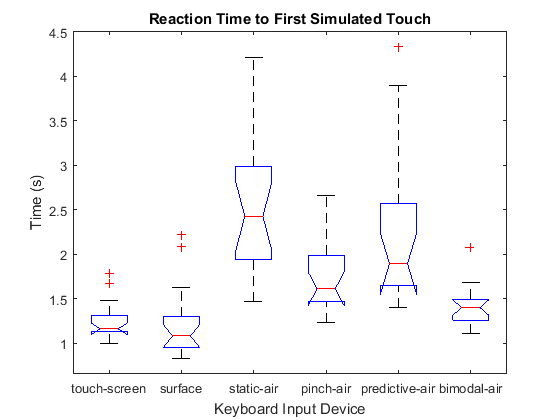
\includegraphics{fig_reaction_touch_boxplot}
	\caption[Reaction Time to Simulate Touch Boxplot]{Median Reaction Time to Simulate Touch for each keyboard showing the 25th and 75th percentiles.}
	\label{fig_reaction_touch_boxplot}
\end{figure}

\begin{table}[h]
\centering
\caption[Reaction Time to Simulate Touch Multiple Comparison]{\centering Tukey's Honest Significant Difference with multiple comparison for Reaction Time to Simulate Touch.}
\label{reaction_touch_multcompare}
\resizebox{\textwidth}{!}{\begin{tabular}{ l l r r r r }
\hline
\multirow{2}{*}{Group 1} & \multirow{2}{*}{Group 2} & Confidience Interval & Mean Difference & Confidience Interval & \multirow{2}{*}{$p$-value} \\
{} & {} & Lower End & $\mu_1 - \mu_2$ & Upper End & {} \\
\hline
touchscreen & surface & -0.5034 & 0.0211 & 0.5456 & 1.0000 \\
touchscreen & static-air & -1.8777 & -1.3532 & -0.8287 & 0.0000 \\
touchscreen & pinch-air & -0.9956 & -0.4711 & 0.0533 & 0.1044 \\
touchscreen & predictive-air & -1.5133 & -0.9888 & -0.4643 & 0.0000 \\
touchscreen & bimodal-air & -0.6888 & -0.1644 & 0.3601 & 0.9431 \\
surface & static-air & -1.8988 & -1.3743 & -0.8498 & 0.0000 \\
surface & pinch-air & -1.0167 & -0.4922 & 0.0323 & 0.0789 \\
surface & predictive-air & -1.5344 & -1.0099 & -0.4854 & 0.0000 \\
surface & bimodal-air & -0.7099 & -0.1854 & 0.3391 & 0.9079 \\
static-air & pinch-air & 0.3576 & 0.8821 & 1.4066 & 0.0001 \\
static-air & predictive-air & -0.1601 & 0.3644 & 0.8889 & 0.3395 \\
static-air & bimodal-air & 0.6644 & 1.1889 & 1.7134 & 0.0000 \\
pinch-air & predictive-air & -1.0422 & -0.5177 & 0.0068 & 0.0552 \\
pinch-air & bimodal-air & -0.2177 & 0.3068 & 0.8313 & 0.5356 \\
predictive-air & bimodal-air & 0.3000 & 0.8245 & 1.3490 & 0.0002 \\
\hline
\end{tabular}}
\end{table}

\clearpage
\subsection{Reaction Time for First Correct Letter}
\begin{figure}[h]
	\centering
	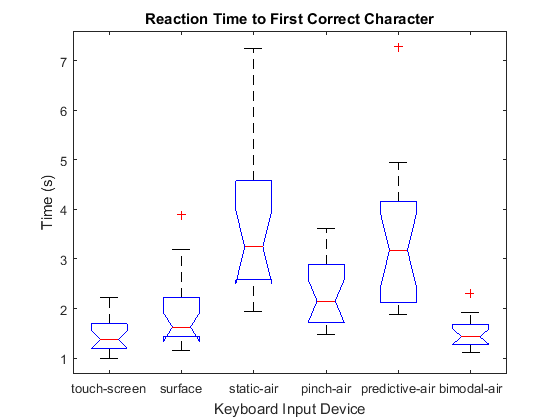
\includegraphics{fig_reaction_pressed_boxplot}
	\caption[Reaction Time for First Correct Letter Boxplot]{Median Reaction Time for First Correct Letter for each keyboard showing the 25th and 75th percentiles.}
	\label{fig_reaction_pressed_boxplot}
\end{figure}

\begin{table}[h]
\centering
\caption[Reaction Time for First Correct Letter Multiple Comparison]{\centering Tukey's Honest Significant Difference with multiple comparison for Reaction Time for First Correct Letter.}
\label{reaction_pressed_multcompare}
\resizebox{\textwidth}{!}{\begin{tabular}{ l l r r r r }
\hline
\multirow{2}{*}{Group 1} & \multirow{2}{*}{Group 2} & Confidience Interval & Mean Difference & Confidience Interval & \multirow{2}{*}{$p$-value} \\
{} & {} & Lower End & $\mu_1 - \mu_2$ & Upper End & {} \\
\hline
touchscreen & surface & -1.4101 & -0.4882 & 0.4337 & 0.6406 \\
touchscreen & static-air & -3.1678 & -2.2460 & -1.3241 & 0.0000 \\
touchscreen & pinch-air & -1.8268 & -0.9050 & 0.0169 & 0.0575 \\
touchscreen & predictive-air & -2.8838 & -1.9620 & -1.0401 & 0.0000 \\
touchscreen & bimodal-air & -0.9788 & -0.0569 & 0.8649 & 1.0000 \\
surface & static-air & -2.6796 & -1.7578 & -0.8359 & 0.0000 \\
surface & pinch-air & -1.3386 & -0.4168 & 0.5051 & 0.7772 \\
surface & predictive-air & -2.3956 & -1.4738 & -0.5519 & 0.0001 \\
surface & bimodal-air & -0.4906 & 0.4313 & 1.3531 & 0.7512 \\
static-air & pinch-air & 0.4192 & 1.3410 & 2.2629 & 0.0007 \\
static-air & predictive-air & -0.6379 & 0.2840 & 1.2059 & 0.9469 \\
static-air & bimodal-air & 1.2672 & 2.1891 & 3.1109 & 0.0000 \\
pinch-air & predictive-air & -1.9789 & -1.0570 & -0.1352 & 0.0149 \\
pinch-air & bimodal-air & -0.0738 & 0.8480 & 1.7699 & 0.0899 \\
predictive-air & bimodal-air & 0.9832 & 1.9051 & 2.8269 & 0.0000 \\
\hline
\end{tabular}}
\end{table}

\clearpage
\section{Quantitative Measures}
\subsection{Number of Touches Simulated}
\begin{figure}[h]
	\centering
	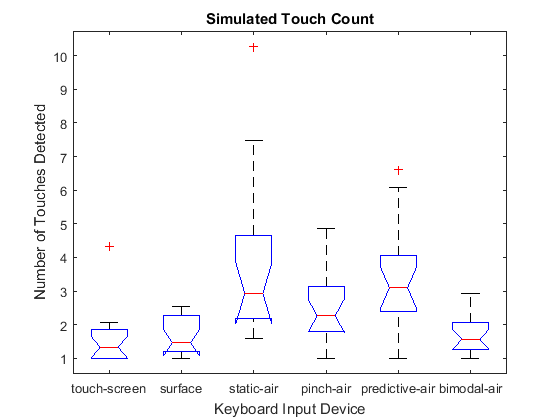
\includegraphics{fig_num_touches_boxplot}
	\caption[Number of Touches Simulated Boxplot]{Median Number of Touches Simulated for each keyboard showing the 25th and 75th percentiles.}
	\label{fig_num_touches_boxplot}
\end{figure}

\begin{table}[h]
\centering
\caption[Number of Touches Simulated Multiple Comparison]{\centering Tukey's Honest Significant Difference with multiple comparison for Number of Touches Simulated.}
\label{num_touches_multcompare}
\resizebox{\textwidth}{!}{\begin{tabular}{ l l r r r r }
\hline
\multirow{2}{*}{Group 1} & \multirow{2}{*}{Group 2} & Confidience Interval & Mean Difference & Confidience Interval & \multirow{2}{*}{$p$-value} \\
{} & {} & Lower End & $\mu_1 - \mu_2$ & Upper End & {} \\
\hline
touchscreen & surface & -1.2824 & -0.0444 & 1.1935 & 1.0000 \\
touchscreen & static-air & -3.4306 & -2.1926 & -0.9546 & 0.0000 \\
touchscreen & pinch-air & -2.0824 & -0.8444 & 0.3935 & 0.3602 \\
touchscreen & predictive-air & -2.9861 & -1.7481 & -0.5102 & 0.0011 \\
touchscreen & bimodal-air & -1.3269 & -0.0889 & 1.1491 & 0.9999 \\
surface & static-air & -3.3861 & -2.1481 & -0.9102 & 0.0000 \\
surface & pinch-air & -2.0380 & -0.8000 & 0.4380 & 0.4222 \\
surface & predictive-air & -2.9417 & -1.7037 & -0.4657 & 0.0017 \\
surface & bimodal-air & -1.2824 & -0.0444 & 1.1935 & 1.0000 \\
static-air & pinch-air & 0.1102 & 1.3481 & 2.5861 & 0.0245 \\
static-air & predictive-air & -0.7935 & 0.4444 & 1.6824 & 0.9022 \\
static-air & bimodal-air & 0.8657 & 2.1037 & 3.3417 & 0.0000 \\
pinch-air & predictive-air & -2.1417 & -0.9037 & 0.3343 & 0.2852 \\
pinch-air & bimodal-air & -0.4824 & 0.7556 & 1.9935 & 0.4878 \\
predictive-air & bimodal-air & 0.4213 & 1.6593 & 2.8972 & 0.0024 \\
\hline
\end{tabular}}
\end{table}

\clearpage
\subsection{Number of Practice Words}.
\begin{figure}[h]
	\centering
	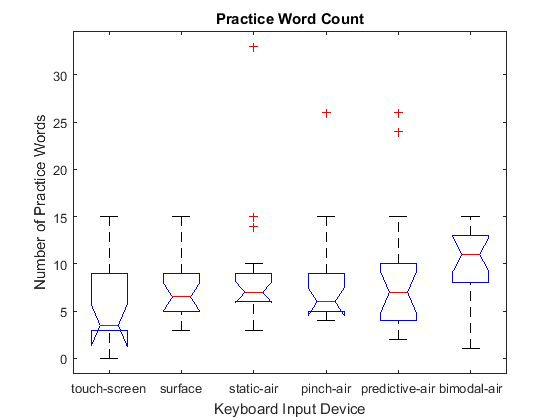
\includegraphics{fig_num_practice_boxplot}
	\caption[Number of Practice Words Boxplot]{Median Number of Practice Words for each keyboard showing the 25th and 75th percentiles.}
	\label{fig_num_practice_boxplot}
\end{figure}

\clearpage
\section{Qualitative Measures}
\subsection{Level of Discomfort}
\begin{table}[h]
\centering
\caption[Level of Discomfort Multiple Comparison]{\centering Tukey's Honest Significant Difference with multiple comparison for Level of Discomfort.}
\label{discomfort_multcompare}
\resizebox{\textwidth}{!}{\begin{tabular}{ l l r r r r }
\hline
\multirow{2}{*}{Group 1} & \multirow{2}{*}{Group 2} & Confidience Interval & Mean Difference & Confidience Interval & \multirow{2}{*}{$p$-value} \\
{} & {} & Lower End & $\mu_1 - \mu_2$ & Upper End & {} \\
\hline
touchscreen & surface & -1.0795 & -0.1667 & 0.7462 & 0.9948 \\
touchscreen & static-air & -2.3573 & -1.4444 & -0.5316 & 0.0002 \\
touchscreen & pinch-air & -1.8573 & -0.9444 & -0.0316 & 0.0381 \\
touchscreen & predictive-air & -2.2462 & -1.3333 & -0.4205 & 0.0007 \\
touchscreen & bimodal-air & -1.3573 & -0.4444 & 0.4684 & 0.7184 \\
surface & static-air & -2.1906 & -1.2778 & -0.3649 & 0.0013 \\
surface & pinch-air & -1.6906 & -0.7778 & 0.1351 & 0.1414 \\
surface & predictive-air & -2.0795 & -1.1667 & -0.2538 & 0.0044 \\
surface & bimodal-air & -1.1906 & -0.2778 & 0.6351 & 0.9496 \\
static-air & pinch-air & -0.4128 & 0.5000 & 1.4128 & 0.6063 \\
static-air & predictive-air & -0.8017 & 0.1111 & 1.0239 & 0.9993 \\
static-air & bimodal-air & 0.0872 & 1.0000 & 1.9128 & 0.0232 \\
pinch-air & predictive-air & -1.3017 & -0.3889 & 0.5239 & 0.8174 \\
pinch-air & bimodal-air & -0.4128 & 0.5000 & 1.4128 & 0.6063 \\
predictive-air & bimodal-air & -0.0239 & 0.8889 & 1.8017 & 0.0610 \\
\hline
\end{tabular}}
\end{table}

\clearpage
\subsection{Level of Fatigue}
\begin{table}[h]
\centering
\caption[Level of Fatigue Multiple Comparison]{\centering Tukey's Honest Significant Difference with multiple comparison for Level of Fatigue.}
\label{fatigue_multcompare}
\resizebox{\textwidth}{!}{\begin{tabular}{ l l r r r r }
\hline
\multirow{2}{*}{Group 1} & \multirow{2}{*}{Group 2} & Confidience Interval & Mean Difference & Confidience Interval & \multirow{2}{*}{$p$-value} \\
{} & {} & Lower End & $\mu_1 - \mu_2$ & Upper End & {} \\
\hline
touchscreen & surface & -1.4179 & -0.3333 & 0.7513 & 0.9475 \\
touchscreen & static-air & -3.4735 & -2.3889 & -1.3043 & 0.0000 \\
touchscreen & pinch-air & -2.6402 & -1.5556 & -0.4709 & 0.0009 \\
touchscreen & predictive-air & -2.5846 & -1.5000 & -0.4154 & 0.0015 \\
touchscreen & bimodal-air & -2.0846 & -1.0000 & 0.0846 & 0.0886 \\
surface & static-air & -3.1402 & -2.0556 & -0.9709 & 0.0000 \\
surface & pinch-air & -2.3068 & -1.2222 & -0.1376 & 0.0177 \\
surface & predictive-air & -2.2513 & -1.1667 & -0.0821 & 0.0273 \\
surface & bimodal-air & -1.7513 & -0.6667 & 0.4179 & 0.4797 \\
static-air & pinch-air & -0.2513 & 0.8333 & 1.9179 & 0.2326 \\
static-air & predictive-air & -0.1957 & 0.8889 & 1.9735 & 0.1729 \\
static-air & bimodal-air & 0.3043 & 1.3889 & 2.4735 & 0.0043 \\
pinch-air & predictive-air & -1.0291 & 0.0556 & 1.1402 & 1.0000 \\
pinch-air & bimodal-air & -0.5291 & 0.5556 & 1.6402 & 0.6728 \\
predictive-air & bimodal-air & -0.5846 & 0.5000 & 1.5846 & 0.7626 \\
\hline
\end{tabular}}
\end{table}

\clearpage
\subsection{Level of Difficulty}
\begin{table}[h]
\centering
\caption[Level of Difficulty Multiple Comparison]{\centering Tukey's Honest Significant Difference with multiple comparison for Level of Difficulty.}
\label{difficulty_multcompare}
\resizebox{\textwidth}{!}{\begin{tabular}{ l l r r r r }
\hline
\multirow{2}{*}{Group 1} & \multirow{2}{*}{Group 2} & Confidience Interval & Mean Difference & Confidience Interval & \multirow{2}{*}{$p$-value} \\
{} & {} & Lower End & $\mu_1 - \mu_2$ & Upper End & {} \\
\hline
touchscreen & surface & -1.2306 & -0.2778 & 0.6750 & 0.9578 \\
touchscreen & static-air & -2.4528 & -1.5000 & -0.5472 & 0.0002 \\
touchscreen & pinch-air & -2.0083 & -1.0556 & -0.1028 & 0.0209 \\
touchscreen & predictive-air & -2.0083 & -1.0556 & -0.1028 & 0.0209 \\
touchscreen & bimodal-air & -1.3972 & -0.4444 & 0.5083 & 0.7535 \\
surface & static-air & -2.1750 & -1.2222 & -0.2694 & 0.0042 \\
surface & pinch-air & -1.7306 & -0.7778 & 0.1750 & 0.1763 \\
surface & predictive-air & -1.7306 & -0.7778 & 0.1750 & 0.1763 \\
surface & bimodal-air & -1.1195 & -0.1667 & 0.7861 & 0.9958 \\
static-air & pinch-air & -0.5083 & 0.4444 & 1.3972 & 0.7535 \\
static-air & predictive-air & -0.5083 & 0.4444 & 1.3972 & 0.7535 \\
static-air & bimodal-air & 0.1028 & 1.0556 & 2.0083 & 0.0209 \\
pinch-air & predictive-air & -0.9528 & 0.0000 & 0.9528 & 1.0000 \\
pinch-air & bimodal-air & -0.3417 & 0.6111 & 1.5639 & 0.4308 \\
predictive-air & bimodal-air & -0.3417 & 0.6111 & 1.5639 & 0.4308 \\
\hline
\end{tabular}}
\end{table}

\clearpage
\subsection{Preference Ranking}
\begin{figure}[h]
	\centering
	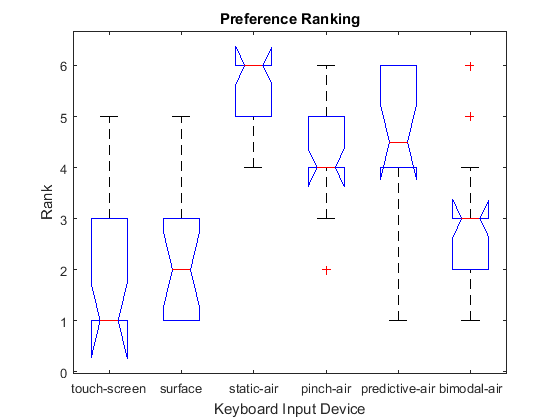
\includegraphics{fig_ranking_boxplot}
	\caption[Preference Ranking Boxplot]{Median Preference Ranking for each keyboard showing the 25th and 75th percentiles.}
	\label{fig_ranking_boxplot}
\end{figure}

\begin{table}[h]
\centering
\caption[Preference Ranking Multiple Comparison]{\centering Tukey's Honest Significant Difference with multiple comparison for Preference Ranking.}
\label{ranking_multcompare}
\resizebox{\textwidth}{!}{\begin{tabular}{ l l r r r r }
\hline
\multirow{2}{*}{Group 1} & \multirow{2}{*}{Group 2} & Confidience Interval & Mean Difference & Confidience Interval & \multirow{2}{*}{$p$-value} \\
{} & {} & Lower End & $\mu_1 - \mu_2$ & Upper End & {} \\
\hline
touchscreen & surface & -2.1104 & -0.3333 & 1.4438 & 0.9948 \\
touchscreen & static-air & -5.2215 & -3.4444 & -1.6673 & 0.0000 \\
touchscreen & pinch-air & -4.1104 & -2.3333 & -0.5562 & 0.0025 \\
touchscreen & predictive-air & -4.3882 & -2.6111 & -0.8340 & 0.0004 \\
touchscreen & bimodal-air & -2.7215 & -0.9444 & 0.8327 & 0.6549 \\
surface & static-air & -4.8882 & -3.1111 & -1.3340 & 0.0000 \\
surface & pinch-air & -3.7771 & -2.0000 & -0.2229 & 0.0169 \\
surface & predictive-air & -4.0549 & -2.2778 & -0.5007 & 0.0035 \\
surface & bimodal-air & -2.3882 & -0.6111 & 1.1660 & 0.9244 \\
static-air & pinch-air & -0.6660 & 1.1111 & 2.8882 & 0.4776 \\
static-air & predictive-air & -0.9438 & 0.8333 & 2.6104 & 0.7648 \\
static-air & bimodal-air & 0.7229 & 2.5000 & 4.2771 & 0.0009 \\
pinch-air & predictive-air & -2.0549 & -0.2778 & 1.4993 & 0.9978 \\
pinch-air & bimodal-air & -0.3882 & 1.3889 & 3.1660 & 0.2251 \\
predictive-air & bimodal-air & -0.1104 & 1.6667 & 3.4438 & 0.0808 \\
\hline
\end{tabular}}
\end{table}
